\section{Introduction}
\label{s:intro}

%\wajih{I have updated the macro logs as it does not make sense to use \ logs for just "system". I have changed the macro to "system logs". Make sure the paper is consistent with that.}

% The effectiveness of IDSes hinges on their ability to accurately detect these threats, maintain low false positive rates, and operate with minimal resource consumption, ensuring system performance is not compromised.

%\wajih{Give the workflow of MSSP and cite that organizations outsource their security. If you find any numbers on how many comapnies use MSSP and outsource their security operations that would be great. If you find any realworld attack examples on MSSP where the data was leaked that would be great as well. }

Intrusion Detection Systems (\ids) are crucial for countering Advanced Persistent Threats (APTs) in enterprises, as evidenced by major attacks, such as Solar Winds~\cite{solarwinds} and NotPetya~\cite{notpetya}. Given their stealth and persistence, many enterprises rely on Managed Security Service Providers (MSSPs) to improve their defenses. A survey~\cite{msspsurvey} involving over 5,000 IT professionals reported that about 75\% of companies use MSSPs. These providers integrate their security systems with clients' systems to manage \logs, typically configuring the clients' systems to transmit \logs to the cloud for analysis. Figure~\ref{mssp} illustrates this MSSP operational architecture.


\begin{figure}[t!]
  \centering
  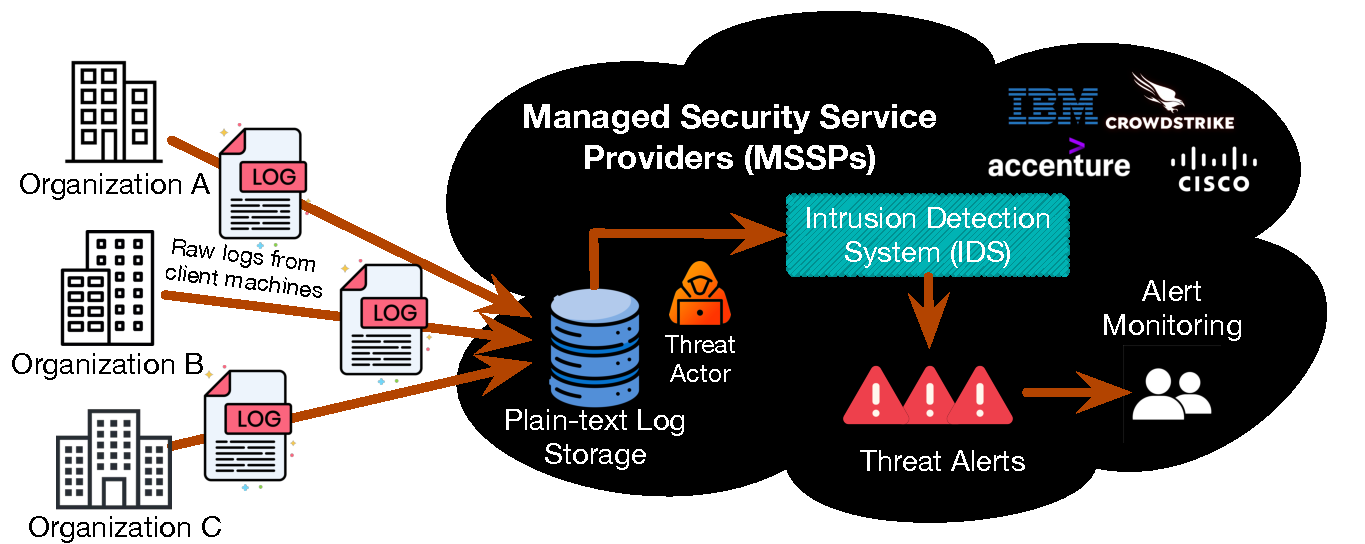
\includegraphics[width=0.32\textwidth]{fig/mssp.pdf}
  \caption{The MSSP architecture for intrusion detection, which is vulnerable to privacy leakage. The plain-text system logs are first collected in a centralized storage managed by the MSSP. Then these system logs are analyzed for intrusions.}
  \label{mssp}
  \vspace{-4ex}
\end{figure}

Recently, Provenance-based IDS (PIDS)~\cite{streamspot,provdetector2020,wang2022threatrace,shadewatcher,yangprographer,han2020unicorn,jia2023magic,flash2024,cheng2023kairos,sigl} have emerged as a highly effective means of enhancing intrusion detection. These systems leverage the extensive contextual information provided by \logs to bolster their detection capabilities. PIDS operates by converting \logs into provenance graphs, which are then analyzed using machine learning techniques, such as Graph Neural Networks (\gnnshort), to identify and learn patterns of benign activity. By continuously monitoring these patterns, PIDS can detect deviations that may indicate potential security threats. Upon detecting such anomalous graph patterns, the PIDS generates alerts to prompt further investigation.


\subsection{Limitations of Existing PIDS}

Despite PIDS potential, the current operational mode of MSSPs and the state-of-the-art PIDS face significant challenges in the complex landscape of enterprise security, which are described below.

\smallskip
\noindent
\textbf{Privacy Risks and Centralized Dependency.} Current PIDS rely on a centralized infrastructure where client machines transmit their logs to a central server. While this centralization is necessary for aggregating large datasets to effectively model and understand benign behaviors using advanced deep learning techniques, it raises significant privacy concerns. Logs often contain sensitive information, such as URLs visited, IP addresses, and application usage, which can be exposed in centralized systems. These privacy risks are not merely theoretical; they have been highlighted in a recent Datadog report~\cite{datadog}. Additionally, training models on data from a single machine is insufficient, as shown by our experiments with \flash on the DARPA OPTC dataset~\cite{darpaoptc}, where performance dropped by 40\% in F-score when using single-host data compared to multi-host data.

    
\smallskip
\noindent
\textbf{Scalability and Operational Inefficiencies}  Centralized PIDS face significant challenges related to both network overhead and scalability. Transmitting large volumes of logs over the network for intrusion detection imposes substantial costs on users and organizations. Modern systems can generate gigabytes of logs daily~\cite{inam2023sok,hossain+depend}. Our analysis of PIDS, such as \flash and \kairos, using the \optc dataset as detailed in Section~\ref{cost_metric}, highlights this issue. For organizations similar in scale to those in the \optc dataset, daily log volumes can reach 1000 GB. This leads to considerable network expenses and difficulties for users with limited bandwidth who struggle to upload such large amounts of logs efficiently. As the number of hosts within an organization increases, centralized PIDS often experience log congestion, creating bottlenecks that slow down intrusion detection. Centralization also results in significant disk storage overhead, requiring continuous resource allocation to manage the growing data. Our evaluations of \flash and \kairos show that these systems would face severe log congestion in environments comparable to the \optc dataset. \flash would require 27.7 hours and \kairos 56.6 hours to process a single day's logs, highlighting the lack of scalability in current centralized PIDS solutions.


\subsection{Our Approach \& Contributions}

We introduce \Sys, a novel privacy-preserving PIDS that integrates provenance graph representation learning with Federated Learning (FL) to address the challenges in applying FL to PIDS. {\it To the best of our knowledge, \Sys is the first system to build a privacy-preserving PIDS and effectively solve these challenges.} \Sys introduces Federated Provenance Graph Learning, combining FL with graph representation learning to create a robust detection mechanism. In \Sys, client logs remain local, ensuring that sensitive data never leaves the client's environment. Each client independently trains \gnnshort models, which are aggregated on a central server with models from other clients. This approach captures diverse activity patterns without transmitting actual logs, minimizing network overhead. Only model updates -- mere kilobytes per client -- are transmitted, greatly reducing the network burden. All major computations, including training, take place locally on client machines, leveraging their resources for real-time threat detection. This decentralized approach allows \Sys to scale effectively as more hosts are added, with each utilizing its own computing power and storage.


However, applying FL to PIDS introduces several significant challenges, summarized below and detailed in Section~\ref{sec:motivation}

\begin{enumerate}[itemsep=0.1em, parsep=0em, topsep=0em]
  \labitem{C1}{itm:c1}{\bf Data Imbalance \& Heterogeneity Among Clients.} Data distribution and volume can vary significantly across clients, complicating the training of a global model that performs uniformly well across all clients. Heterogeneous data distributions from clients running different applications can lead to suboptimal unified model performance~\cite{qu2022rethinking}. Additionally, data imbalances across clients, where smaller data contributors have less impact, can skew learning outcomes~\cite{duan2020self}.

  \labitem{C2}{itm:c2}{\bf Feature Space Heterogeneity.} Inconsistent encoding of identical features across clients leads to difficulties in model convergence and reduces the effectiveness of federated averaging. The independent training of \wordvec models on different client machines results in feature space inconsistencies~\cite{zhou2023fedfa}, complicating the effectiveness of global \gnnshort models.

  \labitem{C3}{itm:c3} {\bf Temporal Misalignment.} Aggregating temporal graph models trained on temporally misaligned data from different clients can result in inconsistencies, impairing the creation of a cohesive global model.
  
  % \labitem{C4}{itm:c4} {\bf Non-Privacy-Preserving Data Structure.} Existing PIDS frameworks often use data structures that do not preserve privacy, making them unsuitable for integration with FL.
\end{enumerate}

\wajih{Make sure that the following paragarphs are correct and have all the information. Very important to highlight all our contributions here. So spend significant time on these paragraphs. Also, make sure to refer C4 and provide solution for that problem.}


To address ~\ref{itm:c1}, we have designed a novel ensemble learning framework. In this framework, each submodel is trained to specialize in learning system activities associated with specific process entities, which are standardized across all clients. This standardization is facilitated by a sophisticated categorization scheme enabled by our dual-server architecture. Through this system, process entities from all clients are organized into \textit{K} privacy-preserving bins. Each client then aligns its process nodes with these bins, constructs a provenance subgraph for each bin, and trains a \gnnshort model on these graphs. The models from all clients are then aggregated into \textit{K} model pairs, forming a comprehensive global ensemble model set. This strategic approach ensures that models with similar data distributions are merged effectively, thereby maintaining the integrity of unique activity patterns across diverse client environments.

To tackle ~\ref{itm:c2}, we implement a \wordvec harmonization scheme utilizing a dual-server architecture. In this setup, a central server issues encryption keys to clients, allowing them to securely encode \wordvec tokens. Subsequently, a utility server processes these encrypted tokens to achieve a unified, privacy-preserving vector representation. This method ensures that sensitive data remains protected while facilitating accurate and consistent semantic encoding across different clients.

To avoid the problem of ~\ref{itm:c3} arising from the use of temporal graph networks, \Sys employs the GraphSAGE~\cite{hamilton2017inductive} neural network, which has been shown by prior work~\cite{flash2024,shadewatcher,wang2022threatrace} to offer good performance and is less affected by temporal dependencies. This approach mitigates the issues of temporal misalignment that often arise in federated learning settings.

\wajih{make sure that the numbers are correct below.}
We conducted extensive evaluations of \Sys using open-source datasets from \darpa, specifically E3~\cite{error3}, E5~\cite{bug5}, and \optc~\cite{anjum2021analyzing}, which encompass a broad spectrum of attack scenarios and system behaviors. The primary goal of \Sys is not to improve the accuracy of state-of-the-art PIDS, but to demonstrate that a privacy-preserving PIDS can be built while maintaining comparable performance. Our results show that \Sys achieves impressive detection performance, with an average precision of 96\% and recall of 97\%, matching the accuracy levels of existing PIDS. What sets \Sys apart is its ability to achieve this accuracy while significantly reducing the privacy risks associated with centralized data collection.

\Sys achieves a 170-fold reduction in communication and storage costs compared to existing systems. Moreover, the decentralized nature of \Sys allows for much faster inference times, completing the full \optc dataset in just 3 minutes, whereas \flash and \kairos require many hours. We present a detailed analysis of the privacy protection of our system in Section~\ref{sec:privacy}. We also provide a comprehensive analysis of our system's resilience against adversarial attacks in Section~\ref{sec:discussion}. \Fix{Add more research questions and their results here.}

% The main contributions of our work are as follows:

% \begin{itemize}[topsep=.1ex,itemsep=-.1ex,leftmargin=*]
%     \item[--] To the best of our knowledge, we are the first to introduce federated provenance graph learning in the domain of IDS with our system, \Sys.
%     \item[--] We have introduced a novel \textbf{ensemble learning} and \textbf{process entity categorization} framework for dealing with diverse heterogeneous client data distributions.
%     \item[--] We developed a sophisticated \textbf{\wordvec harmonization framework} using a multi-server architecture for secure private aggregation of semantic attributes.
%     \item[--] We conduct a comprehensive evaluation of our technique on real-world datasets, demonstrating \Sys's effectiveness in detecting system threats while being scalable and privacy-preserving.
% \end{itemize}

%\url{https://anonymous.4open.science/r/TrustWatch}

% \begin{table}[t!]
%   \centering
%   \scriptsize
%     %\caption{Limitations of existing PIDS. \wajih{Add in caption that which PIDS are not specified in the table and why.}}
%     \caption{Existing PIDS limitations. \flash and \kairos outperform other existing PIDS systems ~\cite{wang2022threatrace,han2020unicorn,streamspot,yangprographer,shadewatcher,provdetector2020}. Also, they all suffer from data privacy leakage issues. Therefore, we have excluded these PIDS from the table. }
%     \setlength{\tabcolsep}{10pt}
%       \begin{tabular}{ | c | c | c | c |}

%         \hline
%              & \bf Data & \bf Network  & \bf Scalability \\
%              & \bf  Privacy & \bf  Overhead &  \\
%         \hline
%         \hline
%         \disdet~\cite{dong2023distdet} & NO                       & LOW      & HIGH       \\
%         \hline
%         \flash~\cite{flash2024}     & NO            & HIGH             & MEDIUM      \\
%         \hline
%         \kairos~\cite{cheng2023kairos}     & NO            & HIGH             & LOW         \\
%         \hline
%         {\bf\Sys}  & YES                & LOW               & HIGH        \\
%         \hline
%       \end{tabular}
%       \label{tab:limitations}
%   \end{table}
